\section{Introduction}

We regard an image $I$ as a function that maps voxels of a rectangular grid \hbox{$\mathcal{L} = \mathrm{Z}_{n_{x}} \times \mathrm{Z}_{n_{y}} \times \mathrm{Z}_{n_{z}}$} to a set $G$ of
possible values called the ``dynamic range'' of $I$. The images we are interested in represent objects in physical space. This means that each point $(i,j,k)$ in the
3-dimensional grid $\mathcal{L}$ is associated to a point $(x,y,z) \in \mathbf{R}^{3}$. When the coordinates of a point
\hbox{$(i,j,k)$} are not integers, the image can still be evaluated at $(i, j, k)$ by interpolation provided
\hbox{$(i,j,k) \in \left[0, n_{x}-1\right] \times \left[0, n_{y}-1\right] \times \left[0, n_{z}-1\right]$}, we denote this ``extended'' dense domain by using the bar decorator:
$\bar{\mathcal{L}}$.\\

The function that maps voxel coordinates of a grid $\mathcal{L}$ to their corresponding coordinates in physical space is an invertible affine transformation. Whenever we talk about
\textbf{a grid} $\mathcal{L}$ we implicitly assume that this $\mathcal{L}$ is associated to a specific grid-to-space affine transformation.
Since our images represent objects in physical space, and these objects are not tied to any specific grid, the same object may be \textbf{sampled} over any grid $\mathcal{L}$.
Note however that, if $\mathcal{A}$ is the grid-to-space affine transformation associated to $\mathcal{L}$, this grid can only sample objects contained in
$\Omega_{\mathcal{L}} = \mathcal{A}(\bar{\mathcal{L}}) \subset \mathbf{R}^{3}$. Since the grid-to-space transformation is invertible, we can, and will, unambiguously talk about the
value of image $I$ at a grid point $u\in \mathcal{L}$ or a point in space $u \in \Omega_{L}$.\\

A diffeomorphism is an invertible and differentiable function whose inverse is also differentiable. A diffeomorphism $\Psi$ is represented by a
deformation field $\phi$ that assigns a displacement vector $\phi(x)$ to each point $x$ such that $\Psi(x) = x + \phi(x)$ (therefore, the zero deformation field $\phi \equiv 0$
represents the identity diffeomorphism). The deformation field itself is defined in physical space and is discretized on its own grid, which of course is associated to
a grid-to-space transform.\\

Let $I, J$ be two images defined over grids $\mathcal{L}_{I}$, $\mathcal{L}_{J}$ with grid-to-space affine transforms $\mathcal{A}_{J}, \mathcal{A}_{I}$, respectively. Let
$\Psi:\Omega_{I} \rightarrow \Omega_{J}$ be a diffeomorphism where $\Omega_{I} = \mathcal{A}_{I}(\bar{\mathcal{L}_{I}})$,
and $\Omega_{J} = \mathcal{A}_{J}(\bar{\mathcal{L}_{J}})$ are the regions of $\mathbf{R}^{3}$ that are sampled by grids $\mathcal{L}_{I}$ and $\mathcal{L}_{J}$, respectively.
To ``warp'' image $J$ towards image $I$, we take each voxel $i \in \mathcal{L}_{I}$ and ``pull''the intensity value of $J$ at its corresponding point in $\mathcal{L}_{J}$
(fig. \ref{fig:pull_back}). More precisely, the warped image $\tilde{J}$ (denoted by the tilde decorator) under $\Psi$, is given by
\begin{equation}\label{eq:warp_definition}
    \tilde{J}(u) = J(\mathcal{A}_{J}^{-1}\Psi(\mathcal{A}_{I}u)), u \in \mathcal{L}_{I}
\end{equation}

\begin{figure}[H]
\centering
\fbox{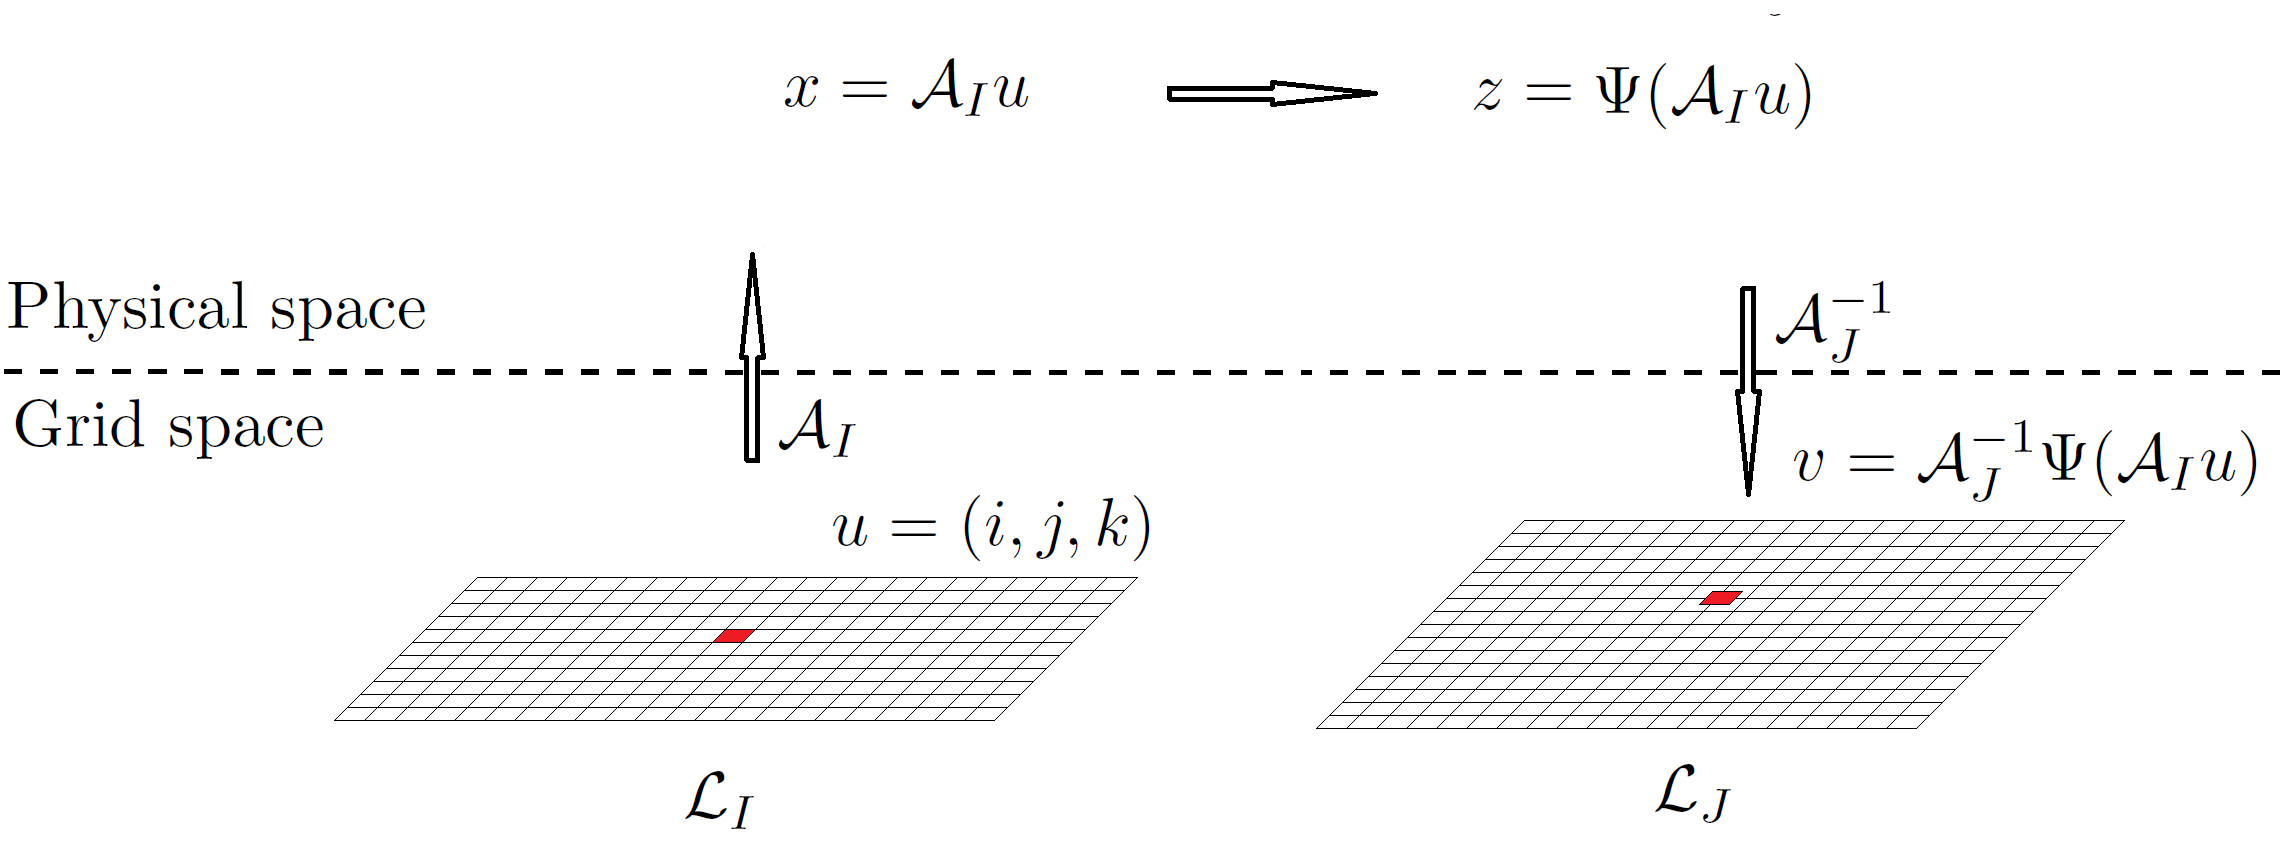
\includegraphics[width=1.0\linewidth]{./images/pull_back.png}}
\caption{Warping an image under a diffeomorphism $\Psi$ is accomplished by ``pulling'' image values at $\Psi$'s codomain towards its domain.}
\label{fig:pull_back}
\end{figure}

\subsection{Symmetric Normalization (SyN)}
The Symmetric formulation for Diffemorphic Image Registration proposed by Avants et al. \cite{Avants2009} consists in minimizing the variational energy given by:

\begin{equation}\label{eq:syn_energy}
    \begin{array}{lll}
        E(I, J) &=& \mathlarger{\int_{t=0}^{0.5} \left\lbrace ||v_{1}(x, t)||_{L}^{2} + ||v_{2}(x, t)||_{L}^{2}  \right\rbrace dt}\\
        &+&\mathlarger{ \int_{\Omega} P(I(\psi_{1}(0.5)), J(\psi_{2}(0.5)), x) d\Omega}
    \end{array}
\end{equation}
subject to
\begin{displaymath}
    \begin{array}{l}
        \frac{d\psi_{i}(x, t)}{dt} = v_{i}(\psi(x,t),t)\\
        \psi_{i}(x, 0) = Id, \psi_{i}^{-1}(\psi_{i}) = Id, \psi_{i}(\psi_{i}^{-1}) = Id, i=1,2,
    \end{array}
\end{displaymath}
where the norm $||\cdot||_{L}$ promotes regularity on the velocity fields $v_{i}$ by penalizing the result of applying the differential operator $L$ (choosen as
$L = \mu \nabla^{2} + \lambda Id$), and $P(I, J)$ is a metric
that measures the dissimilarity between images $I$ and $J$. The {\it symmetric normalization} (SyN) is defined as the solution of the above constrained optimization problem.
The algorithm proposed by Avants et al. \cite{Avants2009}, called {\it Greedy SyN} consists of an unconstrained search within the space of diffeomorphisms with homogeneous boundary
conditions. At each step, the Gready SyN algorithm updates the current estimate of $\psi_{1}, \psi_{2}$ by solving the Euler-Lagange equations defining necessary conditions
that the velocity fields $v_{i}$ must satisfy at each time to minimize eq. \ref{eq:syn_energy}. These equations were provided in \cite{Avants2006} for the Sum of Squared
Differences (SSD) metric as:
\begin{equation}\label{eq:euler_lagrange_ssd}
    Lv = (I - J)\nabla I.
\end{equation}

Equation \ref{eq:euler_lagrange_ssd} is important because it allows us to efficiently solve for $v$ by convolving $(I - J)\nabla I$ with the Green's kernel of the Laplacian $L$, which
is a Gaussian Kernel. Corresponding formulas to efficiently compute the update velocity fields driven by the Cross-Correlation metric were provided in \cite{Avants2009}.
Algorithm \ref{alg:Greedy_SyN} summarizes the Greedy SyN algorithm.

\begin{algorithm}[h!]
\caption{Greedy SyN}\label{alg:Greedy_SyN}
\begin{algorithmic}[1]
\STATE Greedy-SyN algorithm goes here
\end{algorithmic}
\end{algorithm}
